\documentclass[../main.tex]{subfiles}
\begin{document}


In this chapter, we are interested in giving a review of the literature on how to build relational structures automatically. While reviewing pieces of work, we are interested in two aspects: one is the pipeline used to build the relational structure itself, which comprises the mathematical models and algorithms applied to this end, along with their assumptions. If these assumptions are met in our model, then their pipeline or a subset of it could be useful.
\par Additionally, the second aspect of interest are the goals and components of the target relational structure, i.e. the entities and relationships the authors modelled. Discovering links between pairs of bird species is different from segmenting vowel sounds in human speech, for example. Although these differences will probably be reflected in different pipelines, understanding them is key in order to produce a pipeline that will yield better results for our work.
\par However, limiting ourselves to works focusing exclusively on this task might be too restrictive: results from bird classification, clustering and detection could also prove useful for our project. For example, feature extraction is common to all tasks, and state-of-the-art feature extraction is mandatory in order to achieve better results. Therefore, whenever relevant, works on these tasks will also be cited in this review.
\par This chapter is presented as follows: firstly, a general overview of pipelines for building relational structures is given; afterwards, we present a review of feature extraction methods used in acoustic signals; algorithms for building relational structures are reviewed next; finally, a discussion on how the referenced methods are relevant a working pipeline for our scenario is presented.

\section{Relational structures and pipelines}\label{general_pipeline}
A relational structure is one that shows links between objects. In this work, we will assume these links to be a binary relations $R$ over a single set $X$, i.e. $R \subseteq X \times X$. One way of representing such relations is a square matrix $A$, called \emph{adjacency matrix}, such that $A \in \mathbb{R}^{n \times n}$, where $n =\left\vert{X}\right\vert$.
\par In real life, information about objects can be represented as a relational structure. As the number of objects grows large, specific subsets of $R$ may present an increasingly "complex" topology. "Complex graphs" (as they are commonly called in the literature) and how to identify them have been extensively discussed in the field. In \cite{Kim2008}, the authors give a narrowed definition for complex graph, which we adapt as follows:
\theoremstyle{definition}
\begin{definition}{Complex graph}. One such that its topological features deviate from random graphs. In other words, a graph that contains many different subgraphs.
\end{definition}
\par A problem that has attracted attention in recent years is community detection. Given a graph $G = (X, E)$ depicting a relation between pairs of objects in $X$, community detection can be seen as a problem of clustering over $X$, i.e. partitioning the vertices $X$ in such a way that the edges between those in different clusters "are comparatively fewer than those between those belonging to the same cluster" \cite{Fortunato2010}. 
\par Clustering is the task of "grouping or segmenting a collection of objects into subsets or clusters, such that those within each cluster are more closely related to one another than objects assigned to different clusters" \cite{hastie2008}. An example of clustering for the 2-dimensional case can be seen in \ref{clustering}.
\begin{figure}[ht]
\centering
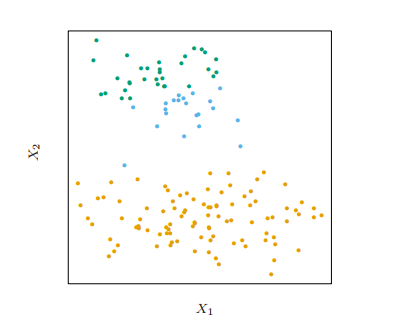
\includegraphics{clustering}
\caption{Simulated data in the plane, clustered into three classes. Image taken from \cite{hastie2008}.}
\label{clustering}
\end{figure}
\par Therefore, performing clustering requires computing the \emph{closeness} of elements in the set of objects $X$. Proximity, closeness, similarity or dissimilarity, all refer to \emph{distance functions} or \emph{measures}. 
\theoremstyle{definition}
\begin{definition}{Measure}.
A non-negative function $d$ satisfying:
\begin{enumerate}
\item Triangle inequality. $d(x, z) \leq d(x, y) + d(y, z) $
\item Symmetry. $d(x, y) = d(y, x)$
\item $d(x, x) = 0$
\item $d(x, y) = 0 \implies x = y$
\end{enumerate}
\end{definition}
\par Thus, defining a measure requires knowledge about what kind of objects we are grouping. In Machine Learning in particular, we will also be concerned by how we transform data into objects for which we can define a measure. This process, called \emph{feature extraction}, consists in "deriving features from raw data that can be used as input for a learning procedure" \cite{hastie2008}. The goal is to use domain knowledge to extract features that will reduce redundancy in raw data and highlight distinguishing characteristics, thus optimising the learning procedure in both, correctness and performance \cite{Bishop2006}. 
\par By working our way backwards, we have implicitly defined a general pipeline to be followed to build relational structures: the algorithms that do so, require the definition of a measure between objects. These objects will be the vectors or features extracted from each object of interest. A diagram depicting this procedure is shown in \ref{pipeline}.
\begin{figure}
\centering
\begin{tikzpicture}[node distance=2cm]
\node (start) [startstop] {Start};
\node (in1) [io, below of=start] {Raw data};
\node (pro1) [process, below of=in1] {Feature extraction};
\node (in2) [io, below of=pro1] {Features};
\node (pro2) [process, below of=in2] {Compute similarity};
\node (in3) [io, below of=pro2] {Pairwise proximity};
\node (pro3) [process, below of=in3] {Build relational structure};
\node (out1) [io, below of=pro3] {Relational structure};
\node (stop) [startstop, below of=out1] {Stop};
\draw [arrow] (start) -- (in1);
\draw [arrow] (in1) -- (pro1);
\draw [arrow] (pro1) -- (in2);
\draw [arrow] (in2) -- (pro2);
\draw [arrow] (pro2) -- (in3);
\draw [arrow] (in3) -- (pro3);
\draw [arrow] (pro3) -- (out1);
\draw [arrow] (out1) -- (stop);
\end{tikzpicture}
\caption{A general pipeline to build relational structures.}
\label{pipeline}
\end{figure}
\par We can now tackle the rest of this literature review as stages that we can put together in order to build relational structures. We will first give an overview of general aspects of birdsong in section \ref{birdsong_review}, aiming to present in a structured manner the data to be analysed in this work. After, we will dedicate a section for each of the processes comprised in the general pipeline. Section \ref{features_review} presents different procedures to extract features from birdsong automatically. Later, section \ref{measures_review} gives a definition of measures frequently used in the literature. Finally, section \ref{algorithms_review} gives an overview of algorithms used to generate relational structures from input vectors and measures.

\section{General aspects of birdsong} \label{birdsong_review}
In this section, we present the concept of birdsong from a biological perspective. We will address this by giving relevant information on the acoustic structure of birdsong, and how it differs from its counterpart, bird calls. Moreover, we also touch on the social and behavioural functions of birdsong and its relation to human speech. Finally, we discuss some arguments regarding the evolution of bridsong through time.
\par There are two ways of acoustic communication among birds: songs and calls. The former "resemble speech in that they are acoustically complex sequences of stereotyped vocal gestures, lasting from seconds to minutes" \cite{Snowdon2013}. On the other hand, bird calls are shorter, consonant-like sounds whose "contribution to nature's music is minimal" \cite{Marler2004}. 
\par From a functional perspective, birdsong is used to defend territories and for mate attraction or competition \cite{Berwick2013} \cite{Naguib2014}, whereas calls are more intimately related to "issues of life and death, such as: predator alarm, the announcement and exchange of food, and the maintenance of social proximity and group composition and integration" \cite{Marler2004}.
\par Birdsongs and bird calls are also different structurally. Biologists have proposed a hierarchical structure of birdsong: a single song is composed of multiple motifs or patterns, each of which is composed of syllables \cite{Snowdon2013}. This structure can be observed in figure \ref{fig_birdsong_structure}. Bird calls, on the other hand, "are often short, monosyllabic, with simple frequency patterning, often delivered in what often appears to be a disorderly fashion" \cite{Marler2004}. Thus, bird calls often lack the hierarchical structure and repetitive patterns that are so distinctive of birdsong. An example of this can be seen in figure \ref{fig_birdcall}.

\begin{figure}[t]
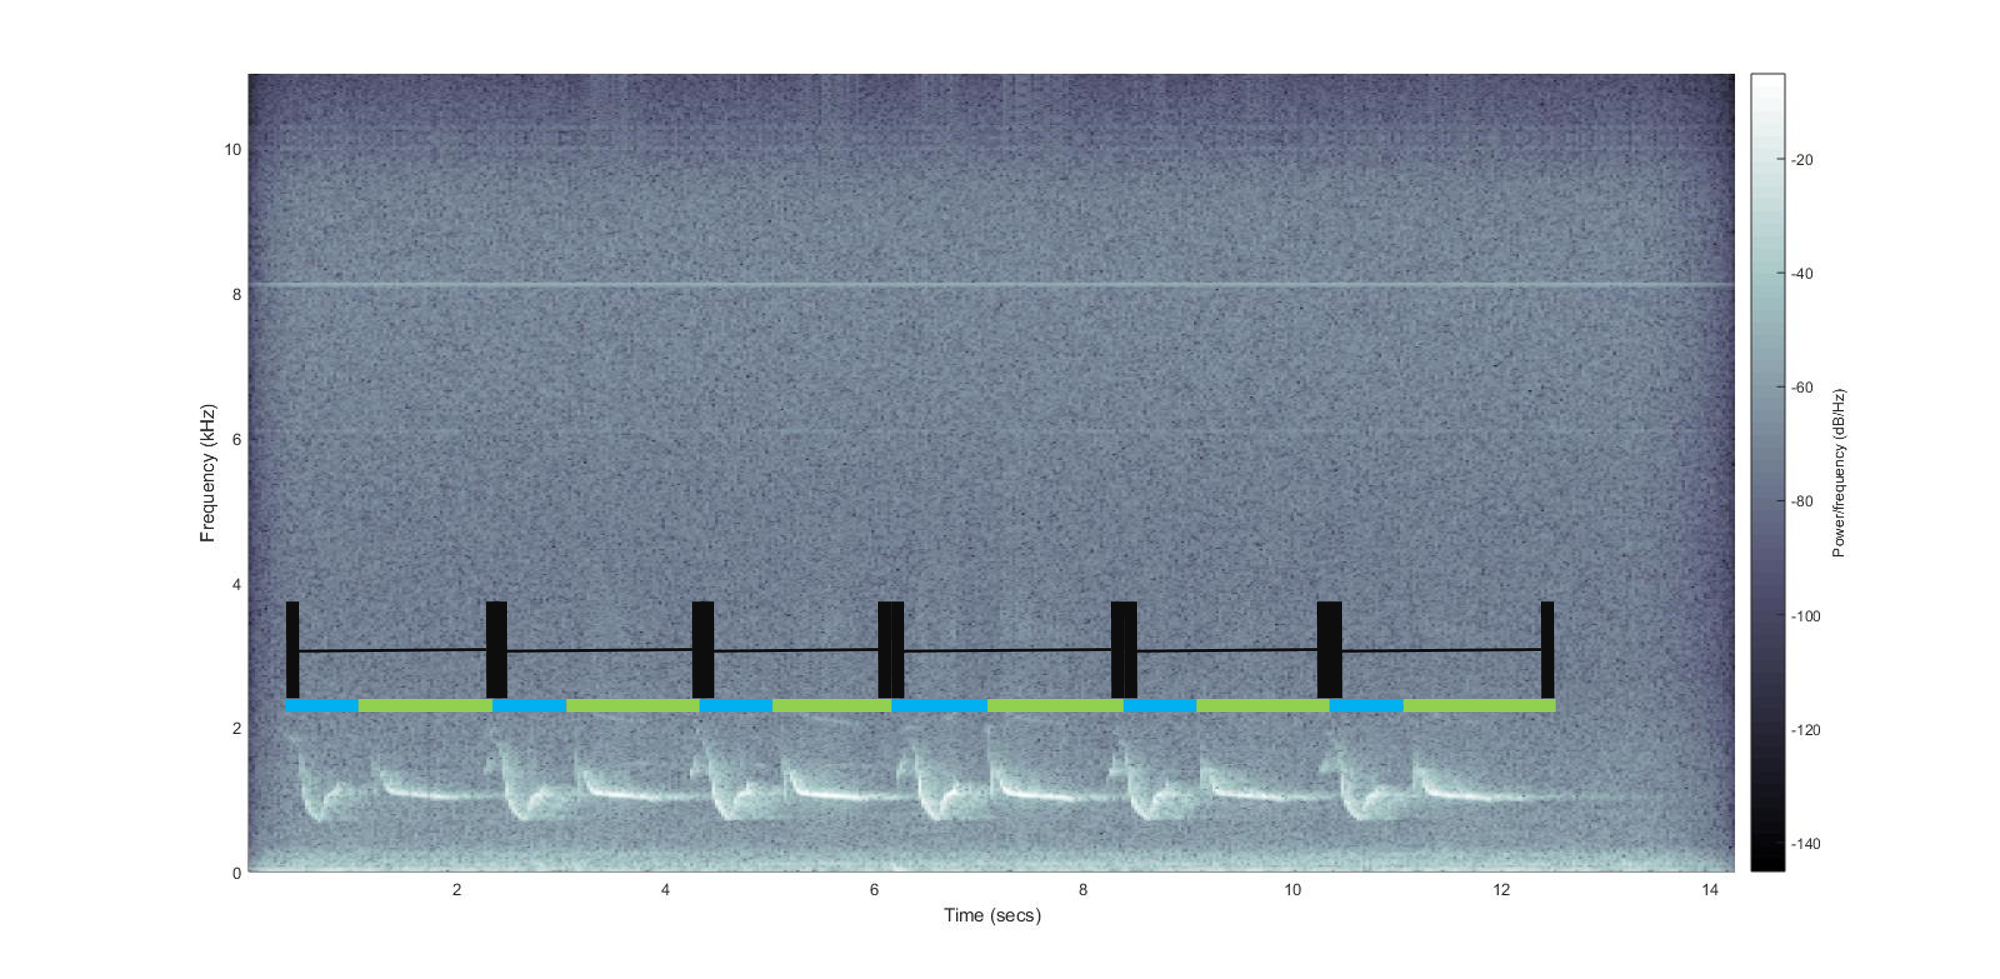
\includegraphics[width=\textwidth]{birdsong_structure}
\caption{Spectrogram from a birdsong recording of the species \emph{Periparus ater}. The thick blue and green bars represent syllables, and the black boxes represent a motif.}
\label{fig_birdsong_structure}
\end{figure}

\begin{figure}[t]
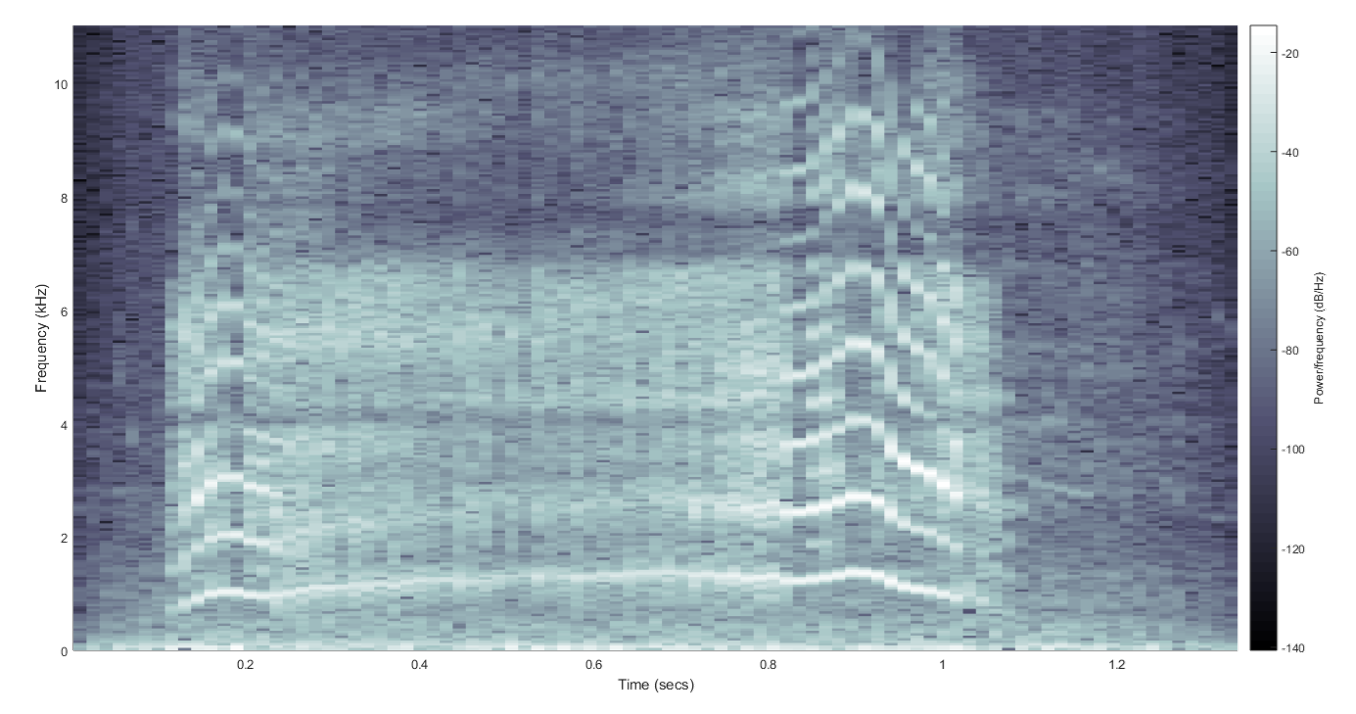
\includegraphics[width=\textwidth]{birdcall}
\caption{Spectrogram from a bird call recording of the species \emph{Vanillus vanillus}.}
\label{fig_birdcall}
\end{figure}

\par In this work, we will be concerned exclusively with birdsong examples. Now that we have compared both types of bird communication, we will focus only on birdsong. The remaining of this section will present more relevant features of birdsong and its association with human speech and evolution.
\par Biologists support the idea that birdsong is learnt by imitation of parent birds \cite{Berwick2013}, i.e. young birds copy many elements of elder birds to produce birdsong. Moreover, the patterns that can be produced by birds can take a long time to master, since birdsong depends on many factors, for example \cite{Naguib2014}: 
\begin{itemize}
\item Some motifs are longer than others, thus mastering them takes longer.
\item Some songs are only produced at a particular time of the day or season of the year.
\item Since one function of birdsong is mating, some songs may only be produced during the birds' fertility period.
\item The energy requirement varies among different songs.
\end{itemize}
\par The fact that birds learn to sing by imitating elder birds is a trait that has caught attention among the field scholars, due to its close relation to how humans learn to speak (by imitation as well). This is not the only similarity between both scenarios: both, birdsong and human language "involve complex, patterned vocalisations" \cite{Berwick2013} \cite{Naguib2014}. The similarity between birdsong and human speech is also related to the auditory system of birds and humans: both hear best between 2 and 5 kHz, unlike other models of animal auditory processing \cite{Snowdon2013}. Furthermore, the bird auditory system can hear frequencies as high as 10kHz, and its human counterpart can do so up to 20kHz \cite{Snowdon2013}.
\par However, biologists consider human speech to be much more complex lexically and semantically \cite{Berwick2013}, i.e. whereas birdsong has two very clear purposes, human speech serves to many more. These functions are closely tied to the highly structured syntactic structures of natural language. Another way to present this point is: the phonetic complexity of both means of communication is not what makes them most distinguishable (both have syllables that make up words), but the idea that human speech adds further levels of abstraction by proceeding to assemble words into sentences, and sentences into full discourses. The morphological, syntactic and semantic complexities of human speech are virtually absent from birdsong. Nevertheless, a strong link still exists in the phonetic abstraction of language.
\par At present, we could make yet another analogy between natural language and birdsong: if human languages have evolved and diversified over time due to sociological and environmental phenomena, how could a similar theory be developed for birdsong, assuming this were even possible? \cite{Cate2004} gives an account of this work stating that past researchers were skeptical about this theory, given that closely related species can diverge strongly in vocal features, just as much as how non-related species could converge in their vocal features due to environmental pressure. The former is more common than the latter, and it occurs often due to acoustic changes occurring in a particular generation, and carried over to the future. Additionally, birds that migrate might be pushed to change the way the sing (or call) due to the presence of new threats. In fact, \cite{Marler2004} states that the loss of natural habitats may actually leave us forever with unanswered questions, precisely due to the missing information that would permit us to trace back the evolution of birdsong.
\par To conclude this section, we point out that more recent research has supported the idea that there is still sufficient information to perform bird species classification \cite{Naguib2014}. Certainly, this is not the same as building a relational structure of bird species, and the arguments above could imply that there is no theoretical guarantee (at least from the biological perspective) that one such relation could exist. However, there is still no guarantee from a statistical or computational perspective that this is indeed the case, and thus Machine Learning becomes relevant to give an opinion on the matter from a mathematical perspective.

\section{Feature extraction procedures for birdsong} \label{features_review}
In this section, we give an account of different birdsong feature extraction techniques used in the literature. Most of these techniques rely on extracting information from the signal in the frequency domain, i.e. if we let a birdsong recording (or a portion of it) be a function of time, namely $x(t)$, then we can take it to the frequency domain and analyse it there. 
\subsection{The Fourier Transform and the FFT algorithm} \label{subsection_fft}
\par One widespread way of performing this domain shift is given by the Fourier transform \cite{Weisstein2015}, defined as:
\theoremstyle{definition}
\begin{definition}{Fourier Transform}.
Given a function $x(t)$, its Fourier transform $X(s)$ is defined as:
\begin{align*}
X(s) = \int_{-\infty}^{\infty}x(t)\mathrm{e}^{-2\pi ist}dx
\end{align*}
\end{definition}
\par We can also define a discrete version of this operation:
\begin{definition}{Discrete Fourier Transform}.
Given a discrete function $\{x_n\}$, its Fourier transform $\{X_k\}$ is defined as:
\begin{align*}
X_k = \sum_{n=0}^{N-1}x_n\mathrm{e}^{-2\pi i\frac{kn}{N}}
\end{align*}
\end{definition}
\par By far the most efficient way to perform the latter is the Fast Fourier Transform (FFT), which runs in $\mathcal{O}(N\log{N})$ \cite{Smith2011}. There are several versions of this algorithm, but one of the most well-known in the literature is the Cooley-Tukey algorithm, described by the eponymous authors \cite{Cooley1965}, \cite{Weisstein2015}. Its general strategy is to use intermediate results in a divide-and-conquer fashion in order to decrease the total number of operations \cite{Weisstein2015}, and it achieves so thanks to the Danielson-Lanczos Lemma:
\begin{lemma}
\emph{Danielson-Lanczos Lemma.} The DFT expansion $\{X_k\}$ of a discrete function $\{x_n\}$ can also be expressed as:\\
\begin{align*}
X_k &= \sum_{j=0}^{N/2-1}\mathrm{e}^{-2\pi i\frac{kj}{N/2}}x_{2j} + W^n\sum_{j=0}^{N/2-1}\mathrm{e}^{-2\pi i\frac{kj}{N/2}}x_{2j+1}\\
&=F^e_k + W^kF^o_k \\
\text{with } W &= \mathrm{e}^ {\frac{-2\pi i}{N} }
\end{align*}
\end{lemma}
\par This is merely regrouping the addition terms as two subadditions, one along the odd-numbered indices, and one along the even-numbered indices. Moreover, by periodicity of the DFT:
\begin{align*}
F^e_k &= F^e_{k+N/2}\\
F^o_k &= F^o_{k+N/2}\\
\mathrm{e}^ {\frac{-2\pi ik}{N} } &= -\mathrm{e}^ {\frac{-2\pi i(k+N/2)}{N} }
\end{align*}
\par This enables us to reformulate the calculation of $X_k$ as:
\begin{align*}
X_k = F^e_k + W^kF^o_k\\
X_{k+N/2} = F^e_k - W^kF^o_k
\end{align*}
\par These reformulations reduce the calculations per recursion to nearly half of the original number, thus resulting in a much better performing procedure. More specific details of this algorithm are beyond the scope of this work, but can be consulted in \cite{Smith2011} and \cite{Cooley1965}.
\par Having discussed the transformation of signals in the time domain into signals in the frequency domain, we are now prepared to set forth different methods of feature extraction.

\subsection{Mel Frequency Cepstral Coefficients (MFCC)} \label{subsection_mfcc}
\par This technique is one of the most widely used in human speech recognition \cite{Jurafsky2009}, \cite{Chou2008a}, \cite{Stowell2014}. It consists in representing the spectral envelope of a frame (a portion of a signal) by analysing its Mel-frequency \emph{cepstrum}. This is done for as many overlapping frames of equal length (around 20-50 milliseconds) that can be extracted from the original signal. The Mel scale is a frequency scale created to simulate how the human ear perceives sounds \cite{Sludge2000}. Its main premise is that human ear perception of pitch is linear below 1 kHz and logarithmic above. In other words, from 1 kHz, the same amount of energy is distributed along longer ranges of frequencies. This results in the human ear having a poorer performance distinguishing very high frequencies.
\par Hertz can be mapped to Mels by the following:
\begin{align*}
F_{\text{mel}} = 1127 \log{(1 + \frac{F_{Hz}}{700})}
\end{align*}
\theoremstyle{definition}
\par We now present the general (scale-independent) definition of the cepstrum, adapted from \cite{Gutierrez-Osuna2009}:
\begin{definition}{Cepstrum} \label{def_cepstrum}
The cepstrum $\V{c}$ of a discrete time signal $\V{x}$ is defined as the Inverse Discrete Fourier Transform (IDFT) of the log-magnitude of the frequency spectrum of $\V{x}$. In other words:
\begin{align*}
\V{c} = \mathcal{F}^{-1}\{\log{(\abs{\mathcal{F}\{\V{x}\}})}\}
\end{align*}
\end{definition}
\par Note that the absolute value $\abs{\mathcal{F}\{\V{x}\}}$ is the square root of the spectral energy of $\V{x}$, which is given by $E(\V{x}) = \abs{\mathcal{F}\{\V{x}\}}^2$. By using the knowledge from the Mel-scale, we can introduce the Mel-frequency cepstrum. The main difference between this and the one from definition \ref{def_cepstrum} is that we compute the magnitude of the spectrum in Mel-scale, rather than in Hertz. Given that the Mel-scale was introduced to model how the human ear detects pitch, this new estimate would show how energy in different \emph{critical bands} of frequencies is being detected by humans. A critical band is a range of frequencies centered around \emph{critical frequencies}, which are distributed according to the Mel-scale, i.e. uniformly before 1 kHz, and exponentially onwards \cite{Gutierrez-Osuna2009}. The length of this range is called the \emph{bandwidth} of the band.
\par In order to estimate the magnitude of the spectrum in Mel-scale, we compute the magnitude of the original frequency spectrum in Hertz and weight it by means of triangular filters along the frequency axis. Each filter corresponds to one critical band, is centered in a critical frequency and the length of its base corresponds to the bandwidth of the critical band, as pictured in figure \ref{mel_energy}.


\begin{figure}[t]
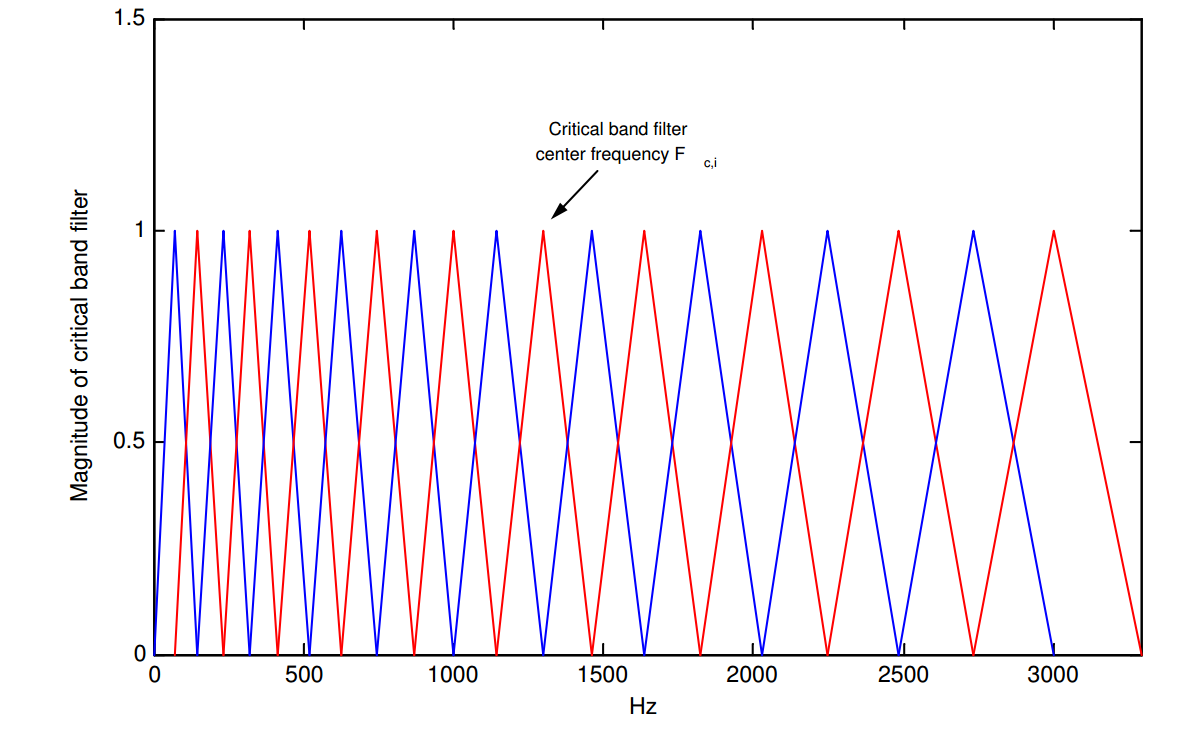
\includegraphics[width=\textwidth]{mel_energy}
\caption{Triangular frequencies to compute the spectral energy in the Mel scale. Picture taken from \cite{Sludge2000}.}
\label{mel_energy}
\end{figure}

\par Then, we continue with the steps described in definition \ref{def_cepstrum}. The result is called Mel-cepstrum and the MFCC are the first $k$ elements of the result. In practice, normally 13 coefficients are taken after using between 20 and 40 triangular filters \cite{Gutierrez-Osuna2009}. However, more recent research has shown that computers now have enough resources to use the full Mel spectrum, rather than just taking the first coefficients \cite{Stowell2014}. Furthermore, MFCC tend to be enhanced with the so-called \emph{delta features}, which represent the rate of change of the MFCC sequence over time \cite{Muda2010} \cite{Lyons2014}. 
\begin{definition}{Delta features.} \label{def_delta_mfcc}
Given a sequence of coefficients $\V{c}$, its delta features are given by:
\begin{align*}
\Delta_t = \frac{\V{c}_{t+1} - \V{c}_{t-1}}{2}
\end{align*}
\end{definition}
\par Similarly, \emph{double delta features} (or acceleration) can be computed by taking the delta features of the delta sequence. 
\par In \cite{Stowell2014}, an analysis of the performance of both, raw Mel spectra and MFCC is presented and compared against other feature extraction procedures when used to characterise birdsong. The conclusion is that, although standard for human speech, there is no proof that this should be the standardised feature extractor for birdsong. The authors present unsupervised feature learning as an alternative that could be more accurate, but call for further benchmarking to be done before coming to an absolute conclusion.

\subsection{Spherical k-means} \label{subsection_spherical}
This is an unsupervised approach to feature learning that consists in finding a normalised spanning set of $K$ vectors for the training dataset. The algorithm was first proposed by \cite{Coates2012}, first used for audio in \cite{Dieleman2013} and in particular for birdsong in \cite{Stowell2014}. It is a modification of the well-known K-means algorithm, where the main difference consists in assigning each datum to the cluster whose centroid produces the minimum cosine distance.
\begin{definition}{Cosine distance} \label{def_cosine_distance}
The cosine distance between two vectors $\V{x}$ and $\V{y}$ separated by an angle $\theta_{\V{x}, \V{y}}$ is given by:
\begin{align*}
d(\V{x}, \V{y}) &= 1 - \cos{(\theta_{\V{x}, \V{y}})}\\
&= 1 - \frac{\V{x} \cdot \V{y}}{\norm{\V{x}}\norm{\V{y}}}
\end{align*}
\end{definition}
\par Moreover, each centroid is normalised at every iteration of the algorithm. The result is a normalised spanning set that displays the directions of greater concentration of data, as depicted in figure \ref{fig_spherical}.

\begin{figure}[t]
\centering
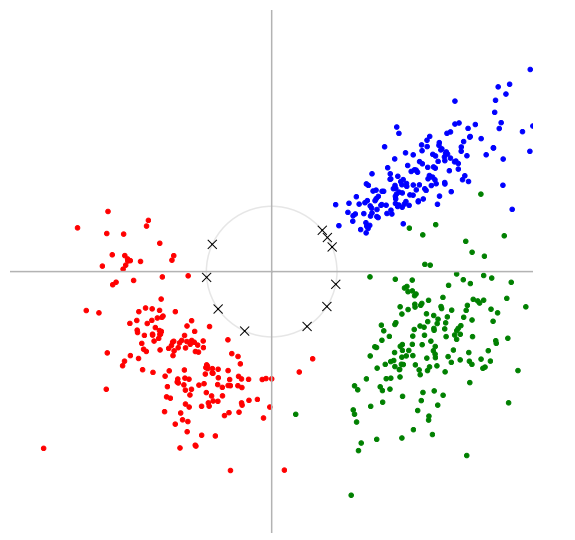
\includegraphics[width=80mm]{spherical}
\caption{Spherical k-means applied to artificial data generated from 3 different 2D-gaussians. The marks represent each of the normalised centroids. Image taken from \cite{Stowell2014}.}
\label{fig_spherical}
\end{figure}
\par The dot product of each datum $\V{x}_j$ with each of the vectors $\V{b}_i$ in the spanning set can be used as features $\V{x}^*_{i,j}$ for a learning procedure, with dimensionality equal to $K$. That is, let $\V{B}$ be the matrix whose rows are the vectors in the spanning set found by spherical k-means, then the new features are given by $\V{x}^*_j = \V{Bx}_j$. In \cite{Stowell2014}, spherical k-means is used as an unsupervised feature extraction procedure for birdsong recordings: the authors used Mel spectral frames (with 40 entries, as described in \ref{subsection_mfcc}) as input to the algorithm. As proposed in \cite{Dieleman2013}, all frames were normalised in length and preprocessed using PCA-whitening. More details of this procedure can be found in \cite{Stowell2014} and \cite{Dieleman2013}.

\subsection{Wavelets} \label{subsection_wavelets}
In this subsection, we give a brief overview of wavelets. This signal analysis technique has been used to analyse birdsong, showing "better results than MFCC" \cite{Chou2009}. Wavelets are an alternative to the Short-Time Fourier Transform (STFT), discussed in subsection \ref{subsection_mfcc}, under the argument that wavelets give better quality results because "they are localised in time and space". This last phrase means that, whereas a small change in the Fourier Transform of a function will produce changes everywhere in its time domain representation (i.e. the FT is only localised in frequency), this is not true for wavelets, since they are localised in both domains \cite{Vidakovic1991}.
\par To expand on this concept, we first introduce orthogonal wavelets.
\begin{definition}{Orthogonal wavelets.} \label{def_onwavelets}
A function $\psi\in L^2(\mathbb{R})$ is called an orthogonal wavelet if the family $\{\psi_{j,k}\}$ is an orthonormal basis for this $L^2(\mathbb{R})$, where each $\psi_{j,k}(t) = 2^{j/2}\psi(2^jt-k)$ and $j, k \in \mathbb{Z}$.
\end{definition}
\par The definition for each $\psi_{j,k}(t)$ arises from the ideas of \emph{binary dilation} and \emph{dyadic translation}: each function has the same shape as the original $\psi(t)$, but has been scaled and translated so as to cover as much as possible from the real line \cite{Chui1992}. 
\par The simplest example of an orthogonal wavelet is given by the Haar function, $\phi_H$ \cite{Chui1992}:
\begin{displaymath}
   \psi_H(t) = \left\{
     \begin{array}{lr}
      1 & 0 \leq t < 1/2 \\
      -1 & 1/2 \leq t < 1 \\
      0 & \text{otherwise} 
     \end{array}
   \right.
\end{displaymath}
\par Now, let $x(t)$ be a signal that belongs to the Hilbert space of square integrable functions, $L^2(\mathbb{R})$ with $\{\psi_{j,k}(t)\}$ as one of its bases. Then $x(t)$ can be expanded as an infinite linear combination:
\begin{align*}
x(t) = \sum_{j,k=-\infty}^{\infty}{c_{j,k}\psi_{j,k}(t)}, \forall j,k \in \mathbb{Z}
\end{align*}

\par Now, the signal can be expanded using a vector of coefficients $\{c_{j,k}\}$. Analogous to the Fourier Transform, we can define a wavelet transform \cite{Weisstein2015a} that will prove useful to solve this problem.
\begin{definition}{Wavelet transform.} \label{def_wtransform} The wavelet transform of a function $x(t)$ with respect to an orthogonal wavelet $\psi$ is given by:
\begin{align*}
(W_\psi x)(b, a) = \abs{a}^{-\frac{1}{2}}\int_{-\infty}^\infty x(t)\overline{\psi(\frac{t-b}{a})}dt
\end{align*}
\end{definition}
\par And the coefficients are given by:
\begin{align*}
c_{j,k} = (W_\psi f)(\frac{k}{2^j}, \frac{1}{2^j})
\end{align*}
\par If we instead approximate the signal $x(t)$ by a finite expansion, then the finite vector of coefficients characterises the signal up to a certain accuracy, and thus can be used as features for a learning algorithm. Finding these coefficients can be solved efficiently using Mallat's Multiresolution Analysis framework. Source \cite{Vidakovic1991} can be consulted for more information on wavelet theory and algorithms.
\par Wavelets have been used successfully in acoustic signal analysis \cite{Gamulkiewicz2003}, and birdsong specifically \cite{Chou2009}. In the former, wavelet transformations are used for speech recognition: each phoneme is used as an input signal, and wavelet coefficients are extracted as features. Phoneme classification is then performed using the Dynamic Time Warping algorithm. 
\par In the latter, wavelet coefficients are used as features to characterise birdsong. However, the wavelet coefficients are not calculated directly: instead, their routine segments the original song into syllables, and then MFCC are calculated for each. The output vectors are treated as input to a wavelet transformation procedure. The result is called WMFCC (Wavelet MFCC). 
\par To conclude this subsection, it must be said that many sources have praised wavelets due to their relative strength over Fourier analysis \cite{Gamulkiewicz2003,Weisstein2015a,Chui1992,Vidakovic1991}; however, implementation issues have also been raised regarding its relative difficult of parametrisation and lack of ability to encode visual energy effectively \cite{Garrett-Glaser2010}.

\subsection{MUSIC algorithm}

\subsection{Formants}
Just describe what formants are and their relationship with LPC models
\subsection{Information geometry}
This brief section deals with how to model other feature extraction outputs as probability distributions or other structures that are learnt.



- MUSIC algorithm
- Principle frequencies as described in \cite{Chou2008}
- Formant
- Information geometry (learning a PDF and using this PDF as input vector)





\section{Measures}\label{measures_review}
\section{Building relational structures}\label{algorithms_review}

\cite{VoVan2010}
N(0) ={W(0)
1 ,W(0) 2 ,...,W(0) n }, with known probability
density functions {f1(x), f2(x), ... , fn(x)}.We partition these populations into progressively inclu- sive clusters, keeping the cluster width at each step minimum. At each step, we only consider the
density functions {f1(x), f2(x), ... , fn(x)}.We partition these populations into progressively inclu- sive clusters, keeping the cluster width at each step minimum. At each step, we only consider the
clusters at the previous step and, from all possible unions, merge the two clusters whose union
has the minimum width. The other clusters do not change.

\cite{Goh2008}
Given a set of pdfs, how do
we develop a computationally simple framework that allows us to group the pdfs into
similar families? Since these pdfs are determined from data, they are non-parametric in
nature.

\cite{hastie2008}
Clustering is the simplest case. K-means. 

\cite{Lu2012}
    The existing community detection methods such as the
diagram segmentation method [2], W-H algorithm [3], hierarchical clustering method [4], and also GN algorithm [1,16], can
only discover non-overlapping community
structure.


\cite{Girvan2002}
The traditional method for detecting community structure in networks such as that depicted in Fig. 1 is
hierarchical clustering. One first calculates a weightWij for every
pair i,j of vertices in the network, which represents in some sense
how closely connected the vertices are.


Edge ‘‘Betweenness’’ and Community Structure.
Instead of trying to construct a measure that tells us which
edges are most central to communities, we focus instead on those
edges that are least central, the edges that are most ‘‘between’’
communities.

\cite{hastie2008}
Divisive clustering
\section{}





Approx. 6K words
What does this chapter contain?

- This should be a literature review. This should firstly give a general overview of approaches people use to build relational structures. This will probably come up to showing that relational structures will usually require a way of representing things (feature extraction) and the definition of a similarity measure, followed by an algorithm that builds a relational structure. A good way of seeing it is backwards: to build a relational structure, we normally require a distance measure, which in turn requires a representation for the objects we are studying. \textbf{provide references for all this reasoning}\\
- Once a general overview has been provided, literature review on each step has to be done. In particular, we care about:\\
- A literature review on feature extraction: again, a general overview of techniques, and a more specific review of what we are using. This means that vector quantisation, MFCCs and formants should all be reviewed.\\
- Talk about dimensionality. It is more useful to have a "general" and "comparable" representation of objects (is is very likely that two different audio recordings will have a different amount of formants, and comparing a subsection of one versus the other might not be ideal. One way of doing this is by learning a more complex, (comparable) structure). There should be a review on KDE and HMM. HMM will probably require an overview of GMMs and Dirichlets, and Variational Inference algorithms\\
- Finally, a review on similarity measures: a brief review of distance measures between probability measures (how are the different from your average measure). KL Divergence, SKLD, Hellinger for KDE. Extend to HMM. Closed forms for 
- How do they build the relational structure? Review on hierarchical clustering


\end{document}